\documentclass[12pt]{article}

\usepackage[margin=1in]{geometry}
\usepackage{setspace}
\usepackage{parskip}
\usepackage{graphicx}
\usepackage{url}
\usepackage{float}
\usepackage{hyperref}


\setlength{\parskip}{0.75em}
\onehalfspacing

\begin{document}
\thispagestyle{empty}

% Custom title page
\begin{center}

    \includegraphics[width=0.5\textwidth]{Logo.png}

    \vspace{2.5cm}

    \textbf{\LARGE American University of Armenia}

    \vspace{1cm}

    \textbf{\Large Integrating Environmental and Hydrological Factors for Accurate Hydropower Generation Forecasting}

    \vspace{1cm}

    \textbf{\large Capstone Project}

    \vspace{1cm}

    DS 299: Capstone

    Spring 2025

    Student: Elvina Nosrati Alamdari

    Supervisor: Aleksandr Hayrapetyan

    \vspace{5cm}

    YEREVAN 2025
\end{center}

\clearpage
\pagenumbering{arabic}
\newpage

% Abstract
\newpage
\thispagestyle{plain}  

\vspace*{0.2\textheight}  

\begin{center}
\section*{Abstract}
\end{center}

\noindent
    
Hydropower plays an important role in renewable energy systems in Armenia and globally. However, it faces several challenges, such as seasonal dependency. This project focuses on three hydropower stations in the Amberd region operated by Amberd LLC, a privately held company. The main challenge in this study was the lack of important variables in the dataset provided by the company. Therefore, estimations and feature engineering techniques were used for accurate forecasting. Statistical methods, machine learning, and deep learning models were examined to predict energy production, with their performance evaluated using standard metrics. The results showed that adding hydrological and environmental features with advanced modeling techniques enhances predictive accuracy. The approach used in this project can help Amberd LLC improve operational planning.

\textbf{Keywoards:} Hydropower forecasting, time-series analysis, deep learning, renewable energy

\newpage
\begin{center}
    \section*{Table of Contents}
\end{center}

\begin{flushleft}
1. Introduction \dotfill \pageref{sec:Introduction} \\
2. Literature Review \dotfill \pageref{sec:Literature Review} \\
3. Methodology \dotfill \pageref{sec:Methodology} \\
\hspace{1em}3.1 Data Collection \dotfill \pageref{sec:data} \\
\hspace{1em}3.2 Data Processing and Feature Engineering \dotfill \pageref{sec:features} \\
\hspace{1em}3.3 Forecasting Techniques \dotfill \pageref{sec:models} \\
\hspace{1em}3.4 Evaluation Metrics \dotfill \pageref{sec:metrics} \\
4. Results and Analysis \dotfill \pageref{sec:results} \\
\hspace{1em}4.1 Exploratory Data Analysis \dotfill \pageref{sec:eda} \\
\hspace{1em}4.2 Model Evaluation Results \dotfill \pageref{sec:ml} \\
\hspace{2em}4.2.1 Machine Learning Models \dotfill \pageref{sec:mlml} \\
\hspace{2em}4.2.2 Shallow Neural Networks \dotfill \pageref{sec:shallow} \\
\hspace{2em}4.2.3 Tabular Deep Neural Networks \dotfill \pageref{sec:tab} \\
\hspace{2em}4.2.4 Time-Series Deep Learning Models \dotfill \pageref{sec:ts} \\
\hspace{1em}4.3 Training Setup \dotfill \pageref{sec:train} \\
5. Discussion \dotfill \pageref{sec:discussion} \\
\hspace{1em}5.1 Evaluation of Findings \dotfill \pageref{sec:evaluation} \\
\hspace{1em}5.2 Conclusion and Future Work \dotfill 
\pageref{sec:limitations} \\
6. Acknowledgments \dotfill \pageref{sec:acknowledgments} \\
7. References \dotfill \pageref{sec:references} \\
\end{flushleft}


\newpage


\section{Introduction}
\label{sec:Introduction}

Hydropower is one of the world's most important renewable energy resources due to its efficiency, which can reach around 90\%. It works by converting the energy of flowing water that comes from either a dam or a river into a turbine that spins to power a generator to produce electricity. Hydropower is highly cost competitive, being the only renewable technology available today that generates electricity at a price equivalent to that of thermal energy sources such as coal, oil, or gas.

The hydropower energy source has several advantages. First, it is a renewable energy source as it depends on the natural water cycle, which means that it can be used repeatedly without disturbing any other resources. Secondly, it is very flexible. It can change its output in minutes, making it a critical tool for grid stability.

Even though this field is widely researched, hydropower forecasting remains challenging, especially in locations with limited data. This is especially true in Armenia, where hydropower plants produce most of their energy during spring and summer due to snowmelt and rainfall. For instance, \textbf{Amberd LLC} generates most of its power from April to August. However, their dataset only includes energy production for 2022-2025, with no data on direct water flow measurements or even environmental data, which are important for accurate forecasting.

Forecasting hydropower stations for companies like Amberd LLC helps in long-term planning by predicting energy demand and identifying potential growing areas. This will allow them to make better investment decisions, such as in the case of Amberd LLC, investing in a reservoir system. So, hydropower companies can improve power generation efficiency, manage supply and demand imbalances, plan economic maintenance activities, engage in energy markets, and make well-informed decisions for long-term sustainability and growth by using various forecasting techniques.

The aim of this research was to see how well forecasting models perform when using derived input features instead of directly measured ones. Results showed that the models using these engineered inputs delivered strong performance. This work may be useful for other energy providers or researchers working with similarly constrained datasets.

\newpage
\section{Literature Review}
\label{sec:Literature Review}
As the global shift toward renewable energy continues, hydropower forecasting becomes an important research area. Many researchers have applied a variety of techniques, from statistical models like ARIMA to more complex deep learning approaches, with recent studies increasingly favoring models that include environmental and hydrological variables as expected.

Despite recent advances, forecasting hydropower generation remains a challenge. However, many studies are based on the assumption that complete weather and inflow data are available. For example, in Zhang et al. (2018) different inflow forecasts were used together (short, medium, long-term) to optimize the real-time operation of a hydropower reservoir. They combined different forecasting models and merged the results using Bayesian theory for better decision-making. Their approach works well with full datasets, but may be hard to apply where data is limited.

Yet, for instance, Li et al. (2015) focused on small hydropower stations, which is important when combining large and medium stations. Their main goal was to reduce water wastage. The results showed that small hydropower plants and large-medium hydropower plants are correlated, which means that when water increases in LHP, it also increases in SHP. With that, they used the forecasted inflow values of large hydropower stations to predict the energy output for small stations. The outcome showed that this method was effective. However, it depends on having complete and reliable data, which we don't have, which is why ML/DL approach is more suitable in our case.

In their study, Stefenon et al.(2023) proposed Wavelet-Seq2Seq-LSTM with Attention model to forecast reservoir levels one hour in advance in hydroelectric power plants. The main idea behind this is to help manage flood risks and maintain operational stability during emergencies. This paper focuses on short-term water level prediction.

Unlike the studies that rely on complete data mentioned before, this study makes forecasts using limited data, which makes it more challenging, which is why instead of relying on direct measurements, water flow was calculated and external weather data was gathered to support forecasting. 

This study contributes to the field by showing a practical forecasting approach designed for real-world data limitations. It evaluates the performance of ML and DL models using engineered features, resulting in accurate hydropower predictions. The implications of these results would be relevant for other researchers or energy providers operating under incomplete datasets or developing systems.


\section{Methodology}
\label{sec:Methodology}

\subsection{Data Collection}
\label{sec:data}

As mentioned previously, the dataset was provided by Amberd LLC, a private energy company operating three hydropower stations in the Amberd region of Armenia. The dataset contains \textbf{hourly energy production values from 2022 to 2025} for all three stations.

To supplement this limitation:
\begin{itemize}
    \item \textbf{Water flow} was \textbf{estimated from energy production} using the standard hydropower formula:\[P = \eta \cdot \rho \cdot g \cdot Q \cdot h\]
    where \( P \) is power, \( \eta \) is efficiency, \( \rho \) is water density, \( g \) is gravitational acceleration, \( Q \) is flow rate, and \( h \) is head~\cite{nascimento2017ridge}.

    \item \textbf{Environmental variables} (temperature, humidity, precipitation) were independently collected from publicly available platforms based on the location and time period of the stations.

\end{itemize}
\subsection{Data Preprocessing and Feature Engineering}
\label{sec:features}

To make the data suitable for modeling, the following steps were applied:
\begin{itemize}
    \item \textbf{Data Cleaning}
    \begin{itemize}
        \item Linear interpolation for small gaps ($\leq$3 days)
        \item Forward-fill for single missing days
    \end{itemize}
    
    \item \textbf{Feature Engineering}
    \begin{itemize}
        \item Lag features: Previous day/week production
        \item Water flow: 3-day/7-day averages and daily/weekly differences
        \item Weather: Temperature deviations, flow-humidity interaction
        \item Seasonal: Monthly cycles (sin/cos)
    \end{itemize}
    
    \item \textbf{Seasonality Analysis}
    \begin{itemize}
        \item STL decomposition for annual patterns
        \item HP filter for trend separation
    \end{itemize}
\end{itemize}

\subsection{Forecasting Techniques}
\label{sec:models}
This study used different forecasting models, including statistical methods, machine learning, and deep learning. Using various models helped to compare their performance in terms of accuracy and interpretability.

\paragraph{1. Statistical Methods}
\begin{itemize}
    \item \textbf{SARIMAX/ARIMA}: Compared performance with and without exogenous weather variables
    \item \textbf{Regularized regression}: Ridge and Lasso as linear baselines
\end{itemize}

\paragraph{2. Machine Learning Models}
\begin{itemize}
    \item \textbf{Tree-based models}: Random Forest, AdaBoost, XGBoost, LightGBM, CatBoost
    
    \item \textbf{Non-linear methods}: SVR and KNN 


\paragraph{3. Deep Learning Models:} Two categories of deep learning models were implemented:

    \item \textbf{Tabular networks}: Shallow FNNs and DeepFNN
    
    \item \textbf{Temporal models}:
    \begin{itemize}
        \item RNN-based: GRU, RNN, BiLSTM, DeepLSTM, Seq2SeqLSTM, CNNLSTM
        \item CNN-based: CNN1D, CNNBiLSTM, GRUCNN
        \item TCN models: TCN, TCNLSTM

    \end{itemize}

\end{itemize}

\subsection{Evaluation Metrics}
\label{sec:metrics}

Model performance was evaluated using the following metrics:
\begin{itemize}
    \item \textbf{Root Mean Squared Error (RMSE)}
    \item \textbf{Mean Squared Error (MSE)}
    \item \textbf{Mean Absolute Error (MAE)} 
    \item \textbf{Coefficient of Determination ($R^2$)} 
\end{itemize}

All models were tested on a 20\% hold-out test set, and models were compared both visually and quantitatively.

\section{Results and Analysis}
\label{sec:results}
\subsection{Exploratory Data Analysis}
\label{sec:eda}
At first glance, there appeared to be some clear seasonal curves in the data with energy production in spring and summer being at its peak(see Fig.~\ref{fig:seasonality}). For a better understanding of how the different variables are linked with each other, the following analyses were carried out:

\begin{itemize}
    \item \textbf{Correlation Analysis:} Pearson correlation matrix was calculated to understand how the different engineered features relate to Normalized Efficiency. The results showed that recent water flow patterns, humidity interactions, and past (lagged) efficiency values were the strongest predictors. (see Fig.~\ref{fig:correlation}).

    \begin{figure}[H]
    \centering
    \includegraphics[width=\textwidth]{seasonality_plot.png}
    \caption{Seasonal pattern observed in daily energy production}
    \label{fig:seasonality}
    \end{figure}

    \begin{figure}[H]
    \centering
    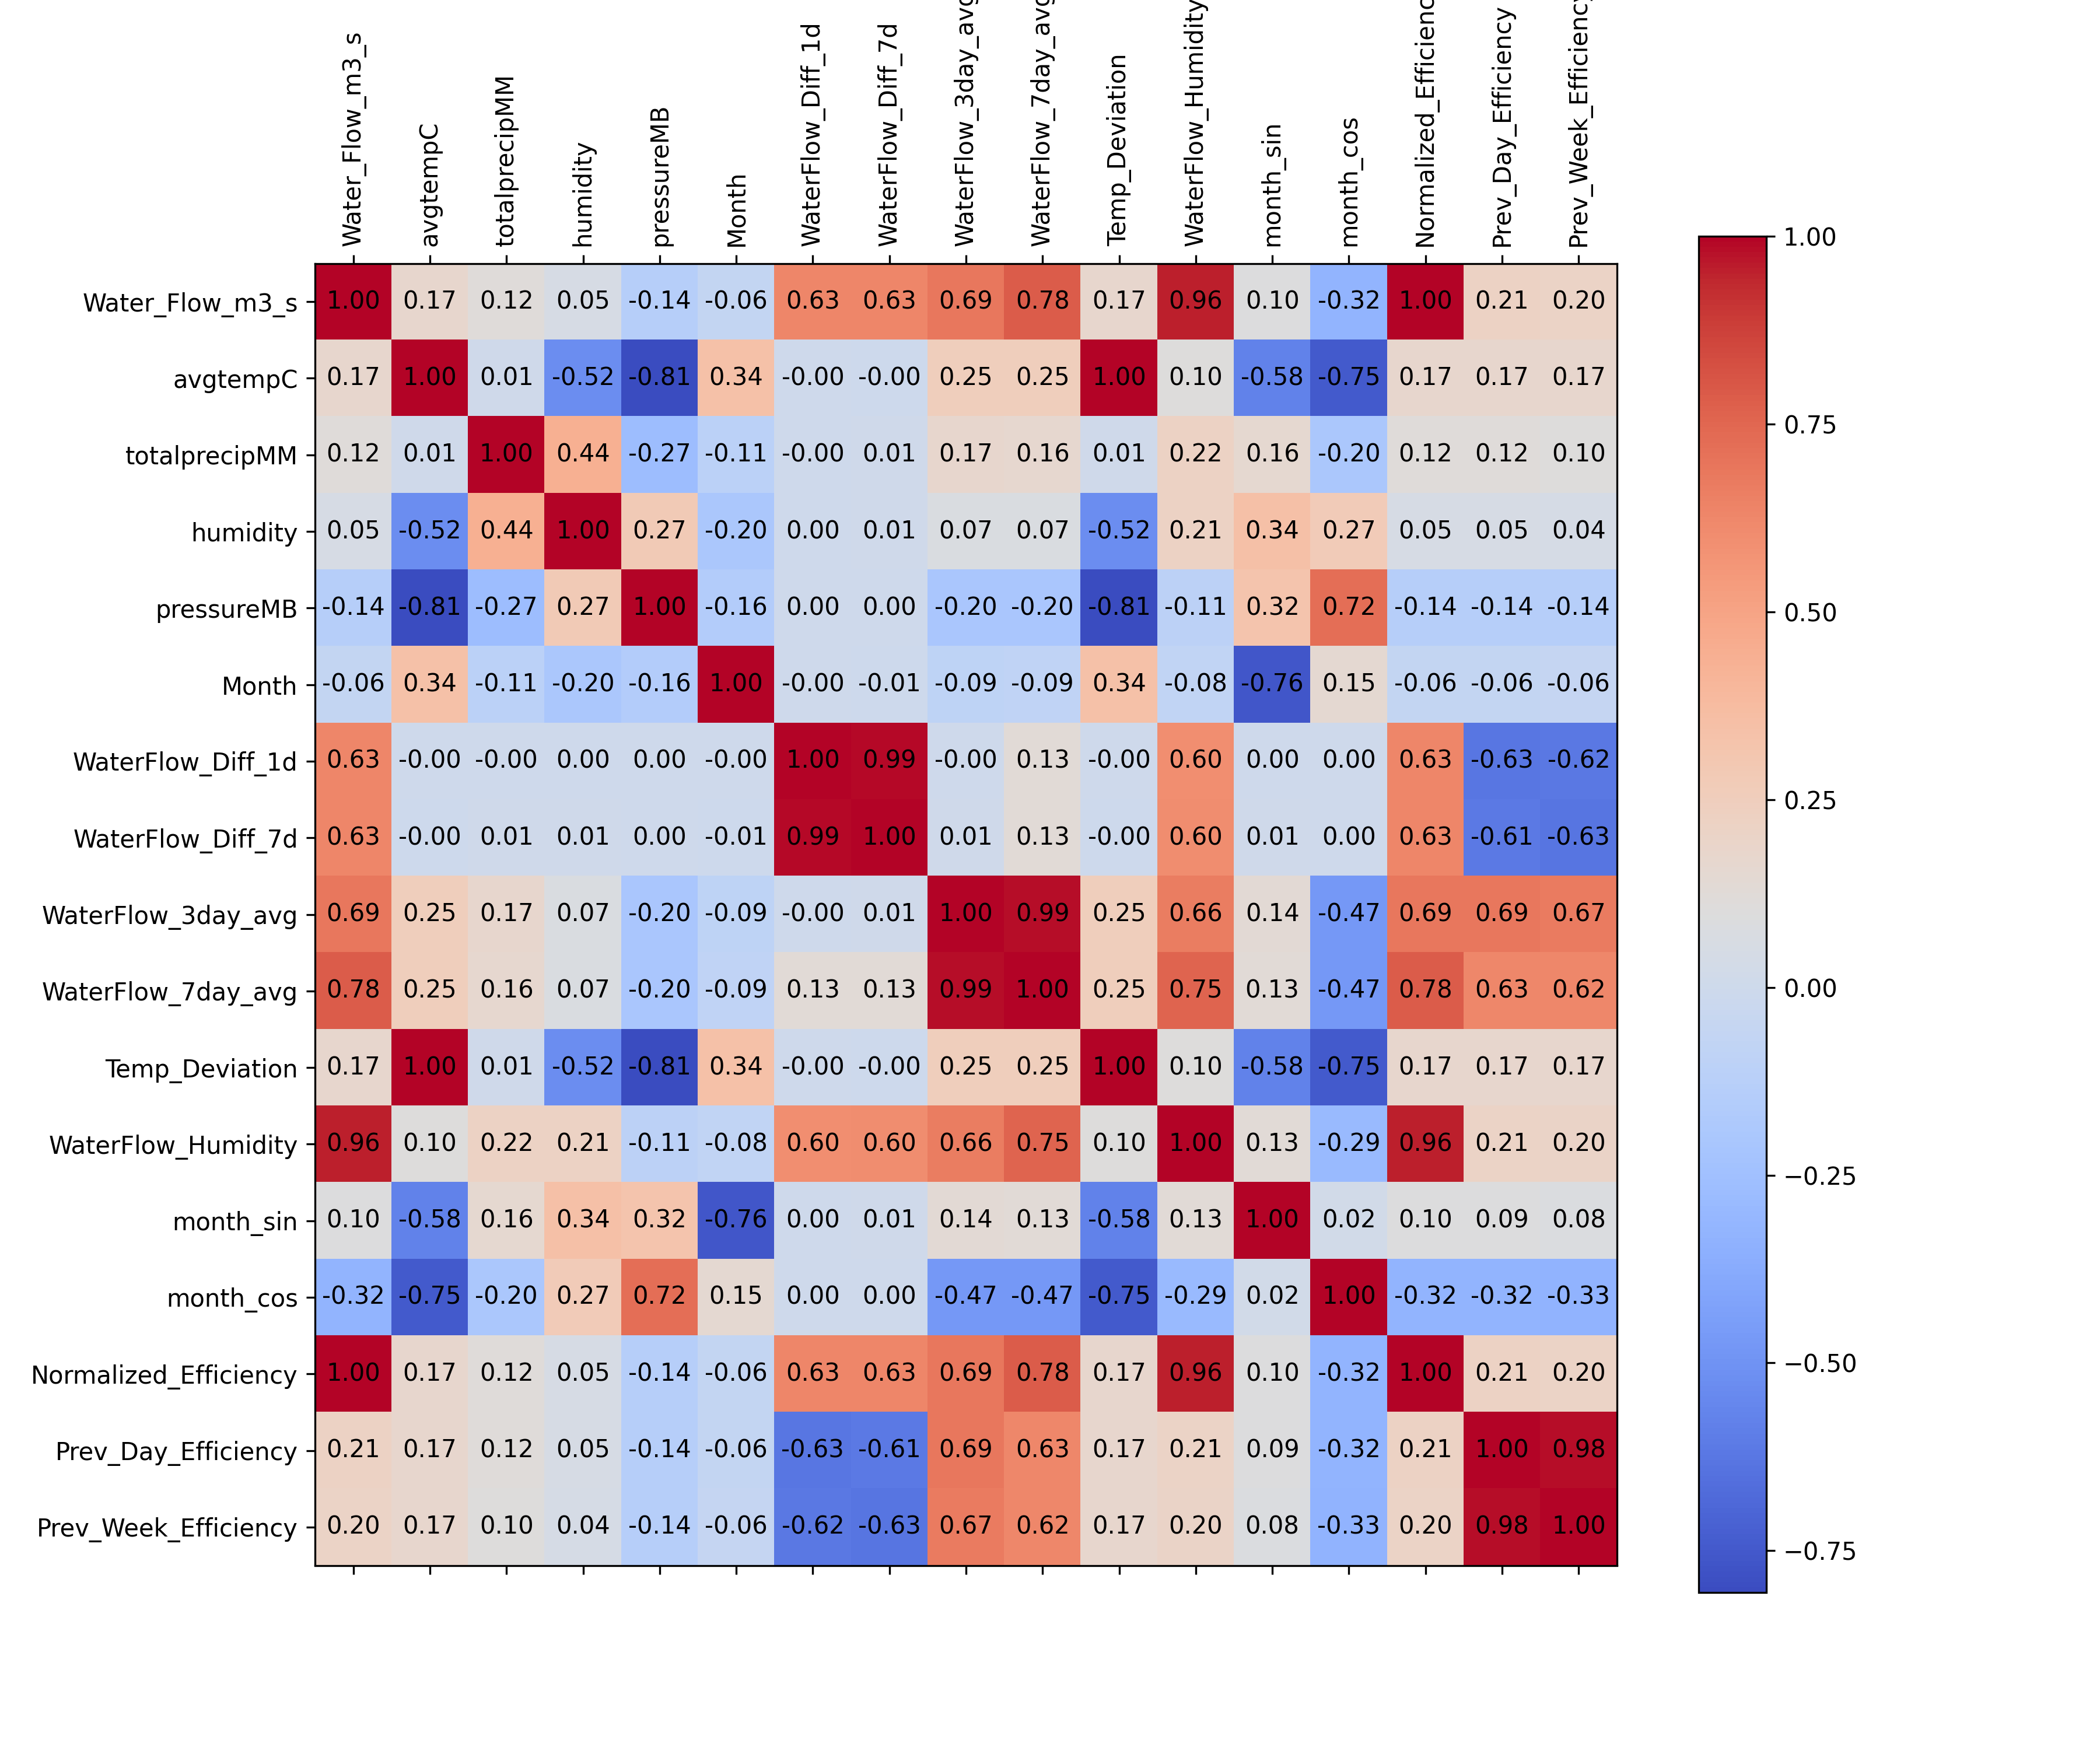
\includegraphics[width=\textwidth]{feature_correlation_matrix.png}
    \caption{Correlation Matrix of Engineered Features and Target Variable}
    \label{fig:correlation}
    \end{figure}
    
    \item \textbf{Seasonal Decomposition:} Severel methods were used for seasonal decompositions, however STL and Hodrick–Prescott outperformed the rest. This helped reveal regular yearly patterns for better model selection.
\end{itemize}

\subsection{Model Evaluation Results}
\label{sec:ml}

\subsubsection{Machine Learning Models}
\label{sec:mlml}
The machine learning evaluation revealed (see Fig.~\ref{fig:ml_metrics}):
\begin{itemize}
    \item \textbf{Tree-based models} dominated, with XGBoost achieving near-perfect $R^2$ (0.999) \cite{chen2016xgboost}
    \item \textbf{Linear models} (Ridge/Lasso) showed theoretical perfect scores \cite{chen2016xgboost}
\end{itemize}

\begin{figure}[H]
    \centering
    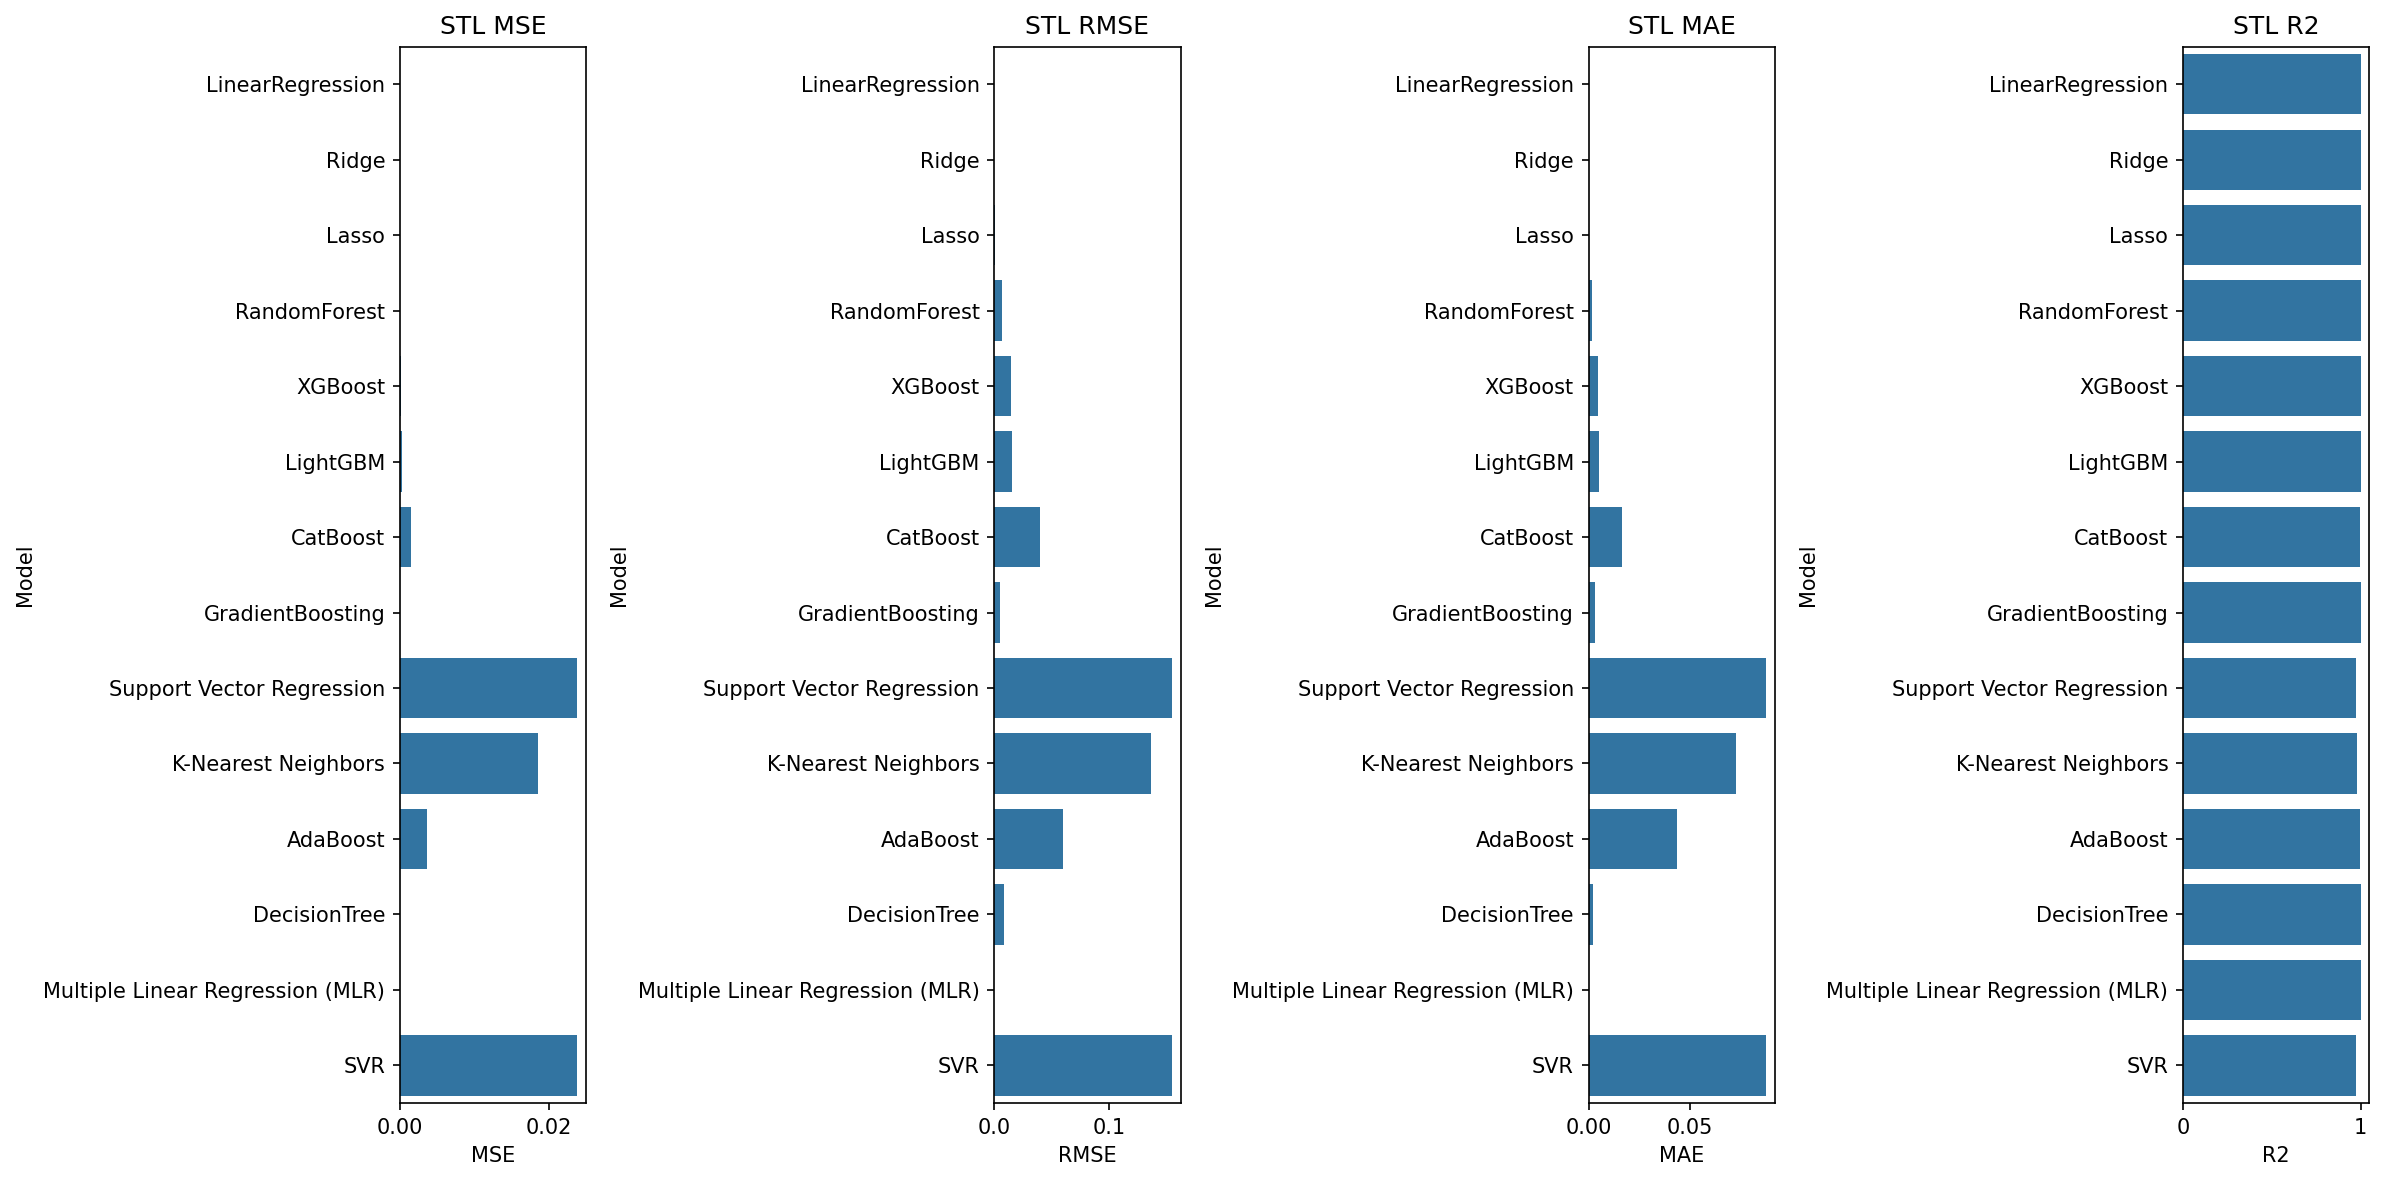
\includegraphics[width=\textwidth]{metrics_barplot.png}
    \caption{Machine Learning Model Performance}
    \label{fig:ml_metrics}
\end{figure}

\textbf{Multiple deep learning models} were implemented for energy prediction forecasting: \textbf{shallow networks}, \textbf{tabular models}, and \textbf{time-series architectures}. The models were chosen based on their ability to learn complex relationships.


\subsubsection{Shallow Neural Networks}
\label{sec:shallow}
Shallow neural networks (Net1--Net4) were developed as baseline models. Each of these architectures consisted of one or two fully connected layers with ReLU activation. These networks remain useful for simple regression task \cite{lecun2015deep}.

To forecast the output for the following day, these models used simple inputs such as energy production, calculated water flow, and hydrological data. Even simpler models, such as Net3, performed surprisingly well (99.9986\% accurate), showing that a moderate depth can be enough to capture relationships in clean, engineered data.

\begin{figure}[H]
    \centering
    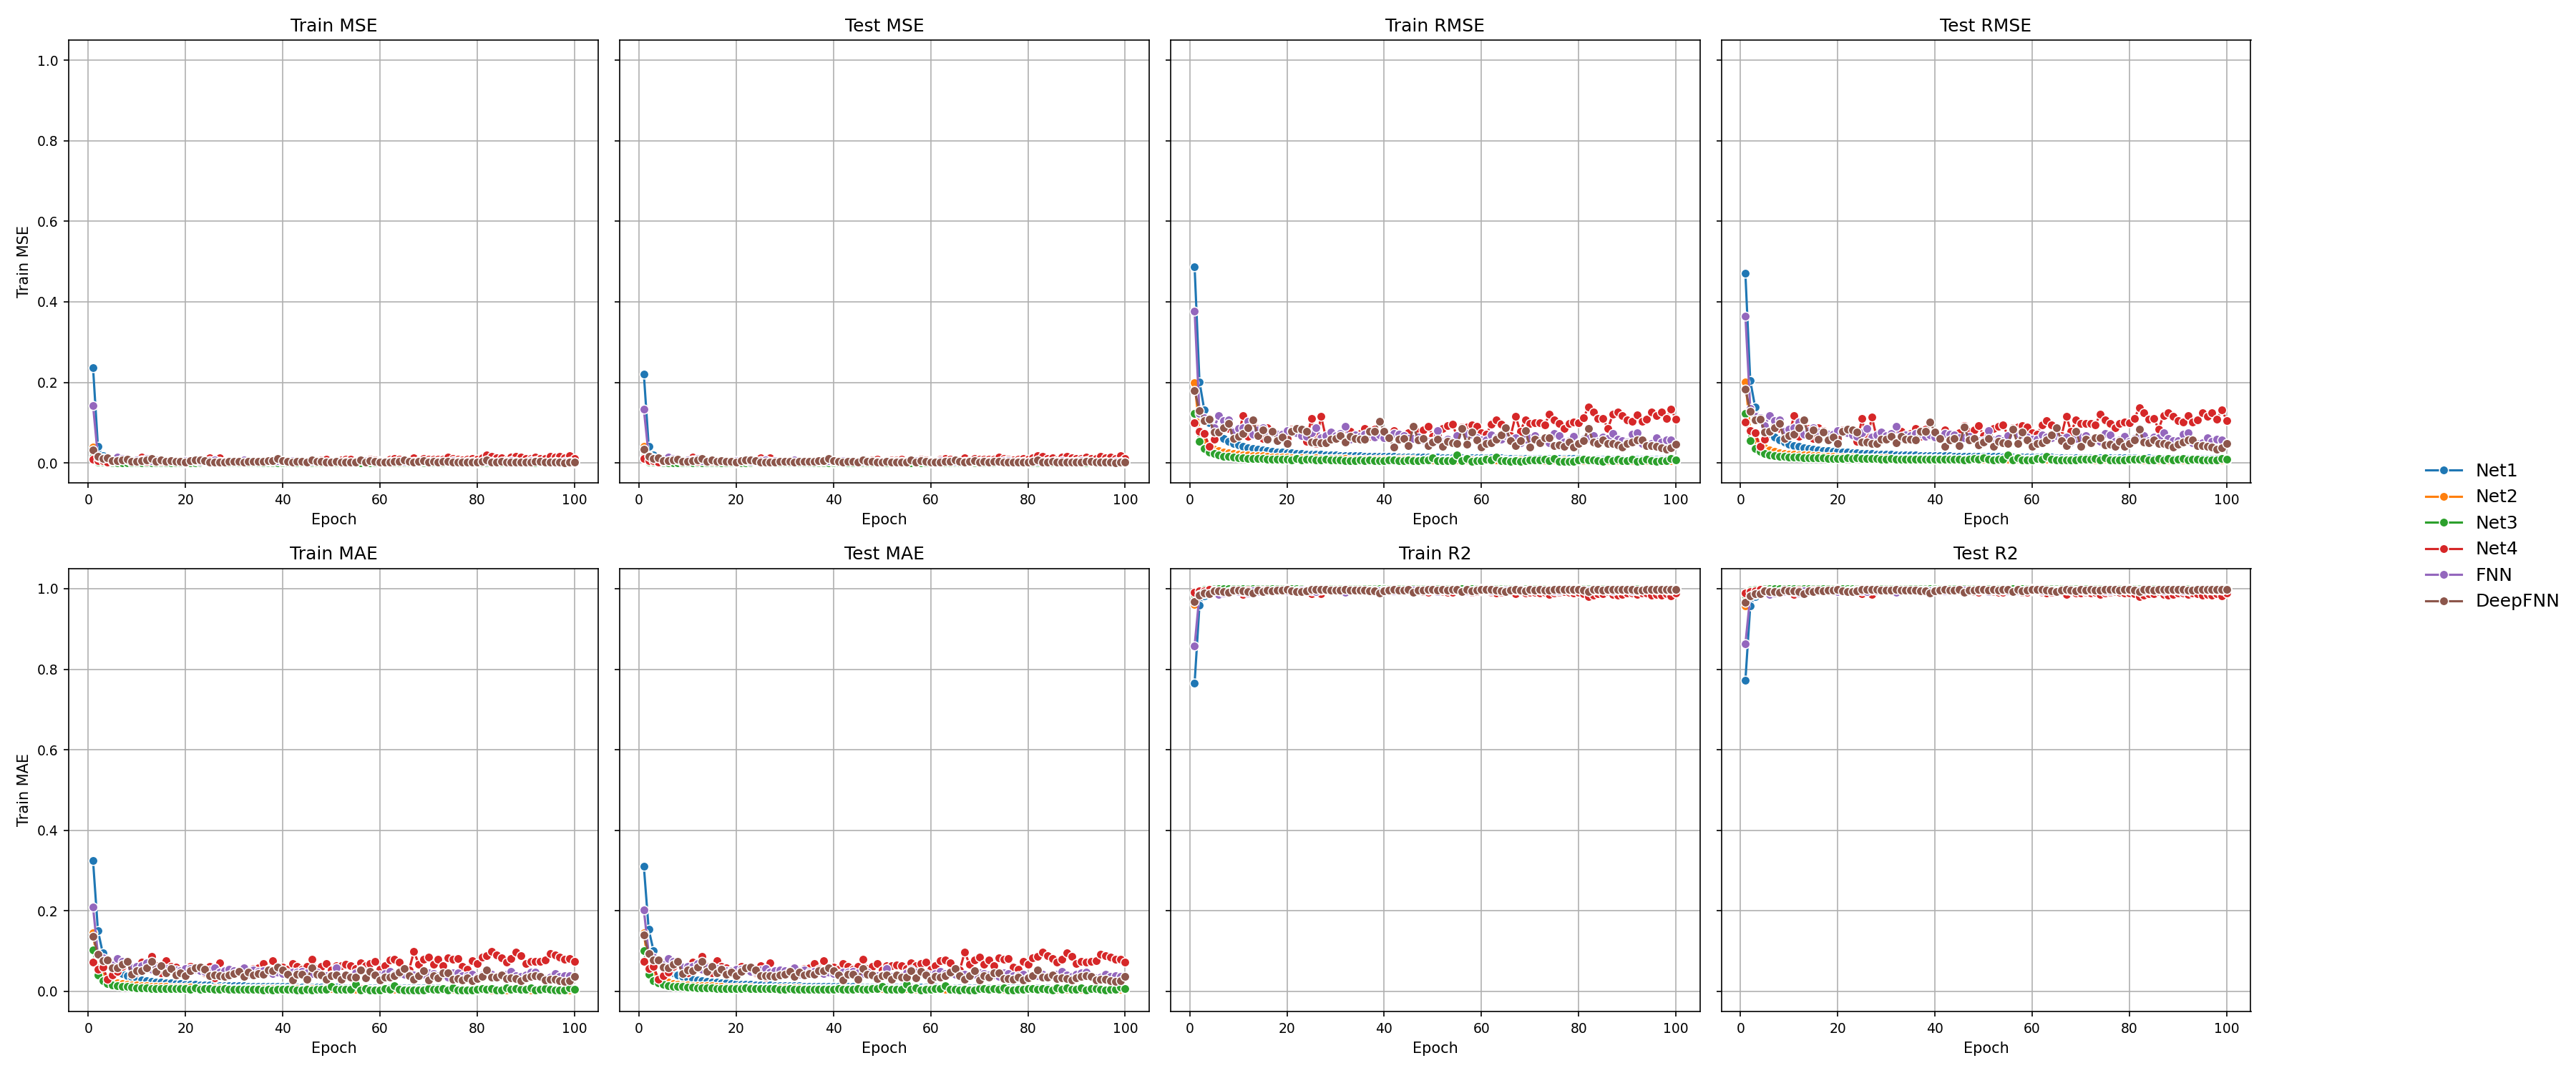
\includegraphics[width=\textwidth]{Train_Metrics_Nets.png}
    \caption{Training and Test Metrics Across Epochs for Shallow Neural Networks}
    \label{fig:net_metrics}
\end{figure}

\subsubsection{Tabular Deep Neural Networks}
\label{sec:tab}

To better capture non-linear relationship between variables, more advanced feedforward models such as FNN and DeepFNN were trained. These models consisted of 3--5 dense layers with ReLU activations and batch normalization \cite{sazli2006, borisov2021}. 

Deeper neural networks (DeepFNN) used the same organized data format as the simpler models, but handled complex real-world variations better, especially when dealing with different stations. The best version scored 99.88\% accuracy, proving that sometimes going deeper helps the model understand trickier patterns.


\begin{figure}[H]
    \centering
    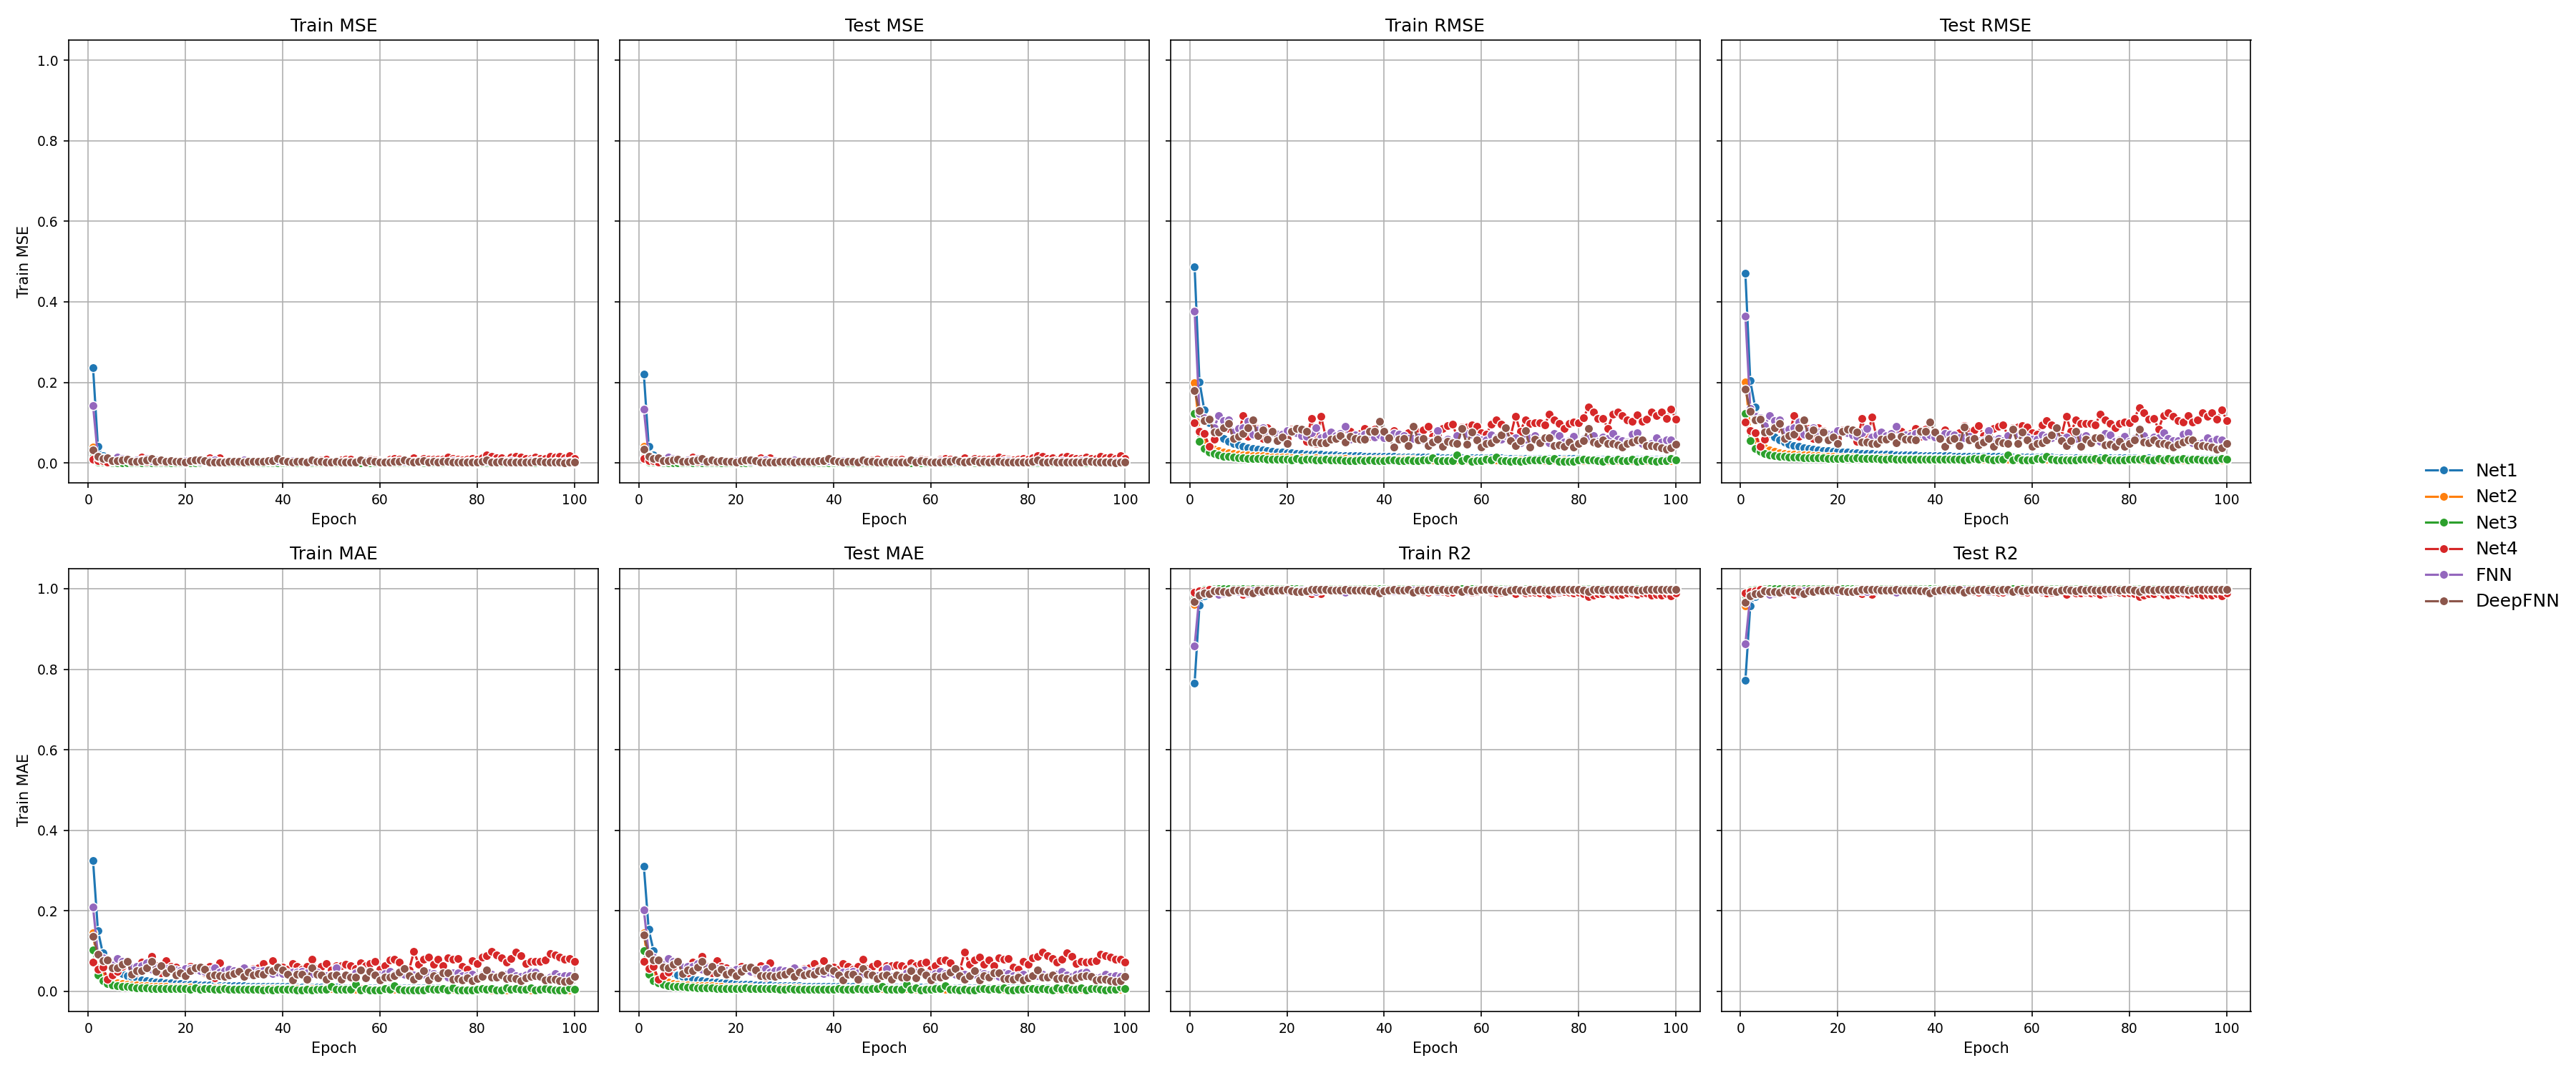
\includegraphics[width=\textwidth]{Train_Metrics_Tabular.png}
    \caption{Training and Test Metrics Across Epochs for Shallow Neural Networks}
    \label{fig:net_metrics}
\end{figure}

\subsubsection{Time-Series Deep Learning Models}
\label{sec:ts}
\textbf{RNN models} can identify sequential features in the data and assist in predicting the next likely data point in the data sequence~\cite{das2023rnn}. In this study, the following RNN-based models were used: basic RNN, GRU, which works similarly as RNN, just trains faster, BiLSTM that reads input forwards and backwards and DeepLSTMNet, which uses multiple LSTM layers for depth. Additionally, hybrids, such as CNNLSTM and Seq2SeqLSTM, were used to see if merging different models could outperform standard models.
    
\textbf{CNN} detects short-term energy patterns  \cite{brownlee2020cnn}. This study extended its capability with hybrid models: CNNBiLSTM, that combines CNN's ability to spot local energy patterns with BiLSTM's bidirectional context analysis and GRUCNN, which combines CNN's ability to detect daily production spikes and GRU's efficient memory.

\textbf{TCN} is easy to compute and it extracts long-term patterns using residual blocks and dilated causal convolutions. This study compared standard TCN against a TCNLSTM hybrid, combining TCN's computational efficiency with LSTM's temporal memory. \cite{lara2020tcn}.
    

\begin{figure}[H]
    \centering
    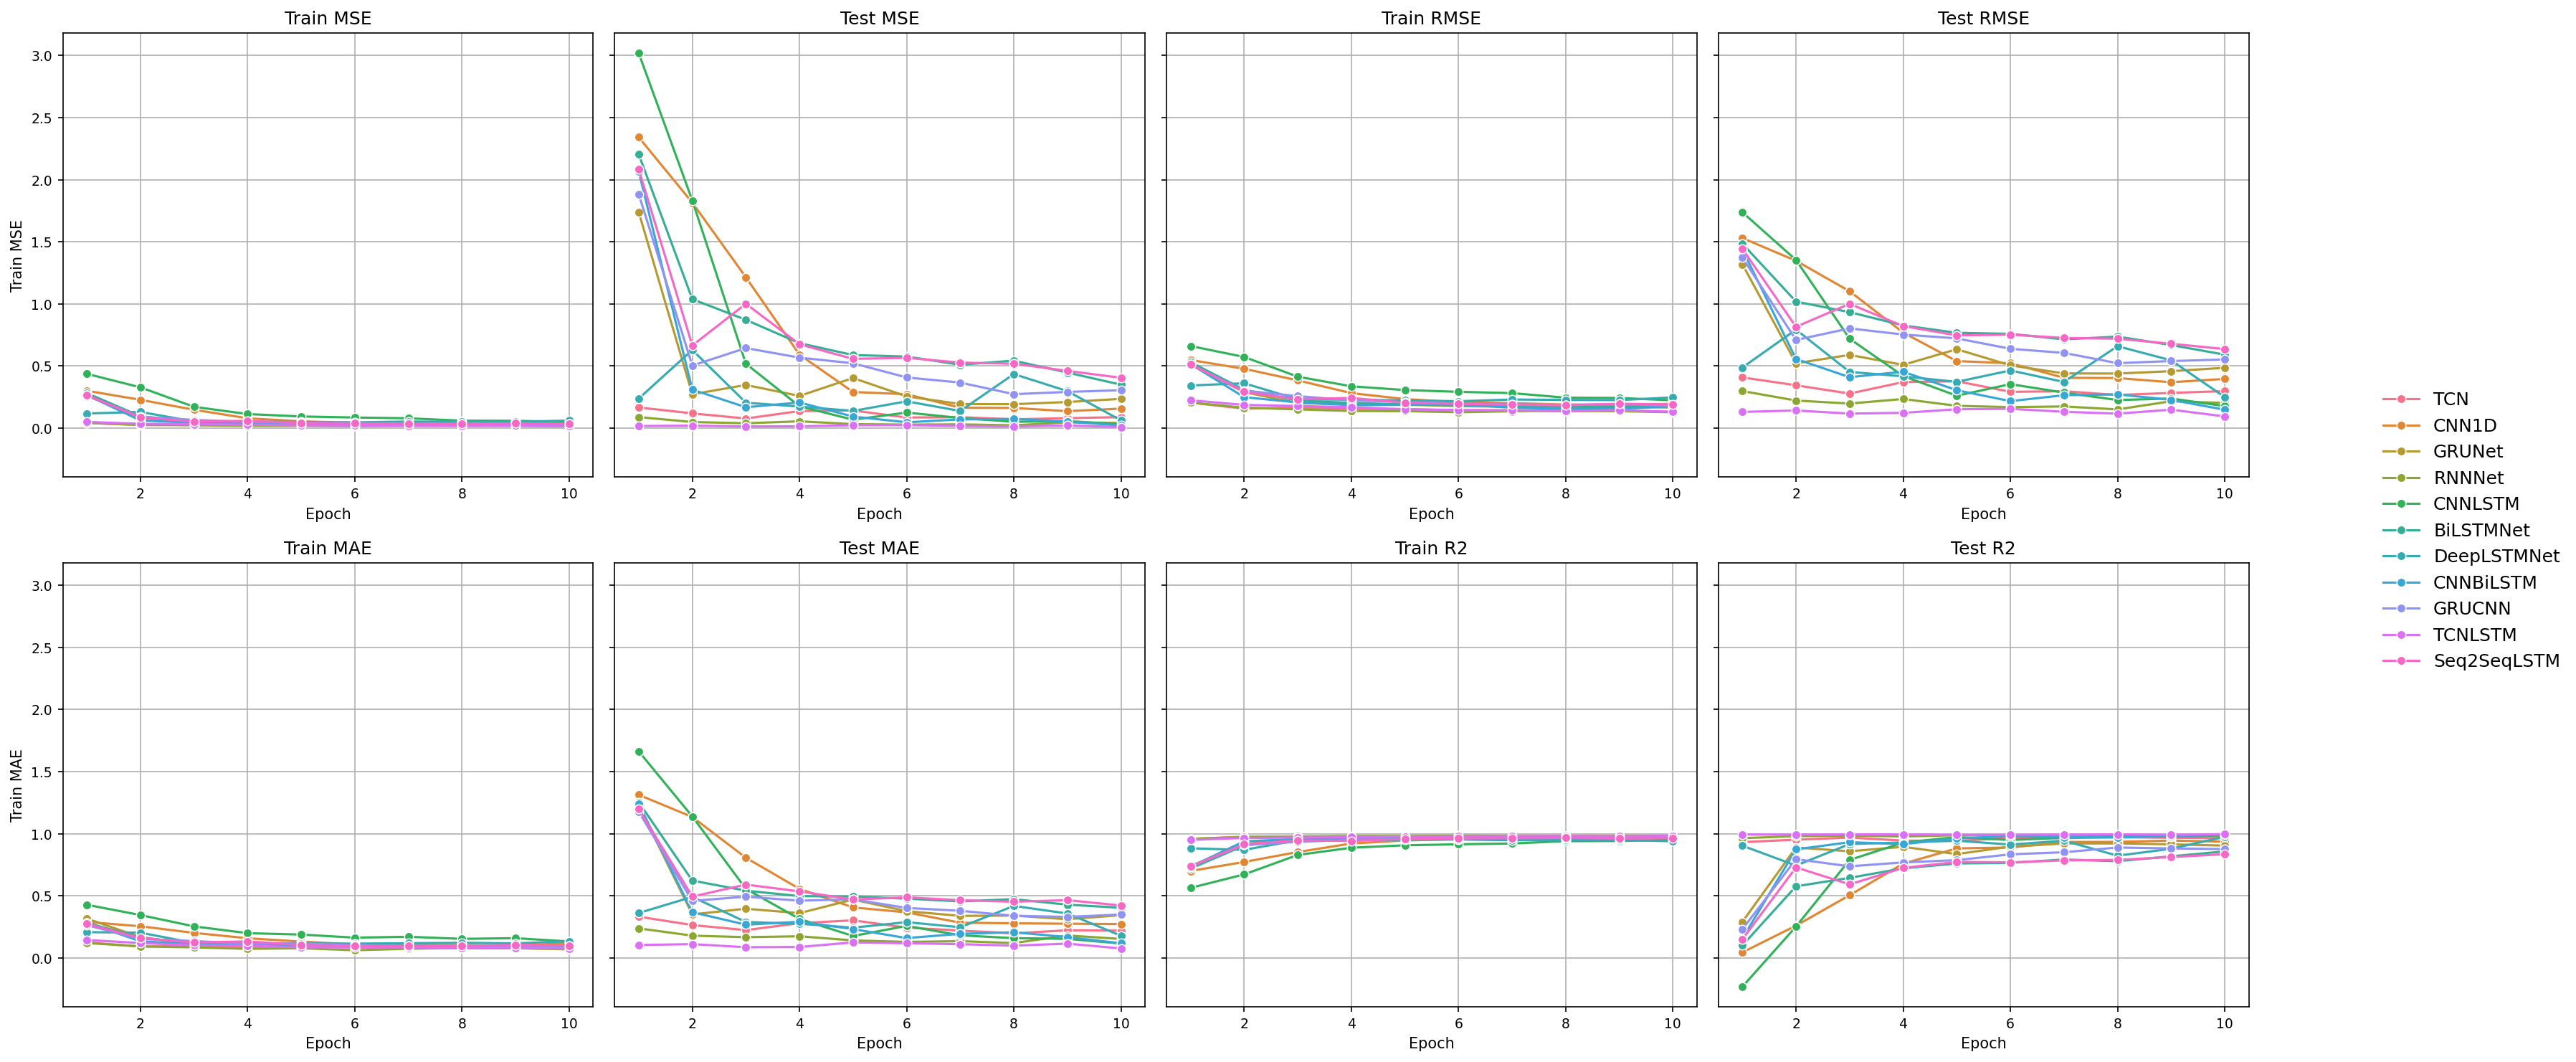
\includegraphics[width=\textwidth]{Train_Metrics_TS.png}
    \caption{Training and Test Metrics Across Epochs for Time-Series Deep Learning Models}
    \label{fig:ts_dl_metrics}
\end{figure}


\subsection{Training Setup}
\label{sec:train}
All deep learning models shared a consistent training framework: Mean Squared Error (MSE) as the loss function, Adam optimization with a learning rate of 1e-3, and a batch size of 32. Shallow networks were trained for up to 1000 epochs, while time-series models used a maximum of 200 epochs.

\section{Discussion}
\label{sec:discussion}

The aim of this paper was to improve hydropower forecasting by combining engineered environmental and hydrological features that focuses only on the three stations operated by Amberd LLC. The results show that both machine learning and deep learning models are capable of giving strong prediction performance even with the lack of direct water flow or hydrological variables. Top-performing models such as Net3, TCNLSTM, and XGBoost tended to reach $R^2$ scores higher than 0.99, showing that derived features and additional weather data can effectively substitute missing variables effectively.

\subsection{Evaluation of Findings}
\label{sec:evaluation}

The evaluation shows three important outcomes. First, deep learning models, particularly TCNLSTM, Net3, and GRUNet established high performance. They capture long-term seasonal trends and short-term operational patterns. Second, machine learning models like Ridge Regression, XGBoost, and LightGBM also achieved high accuracy, however in the seasonal forecasting, they show limitations in complex areas.

More importantly, this study shows how combining engineered features and calculated water flow helps enhance the forecast performance. This approach proves that even with limited or incomplete data it is still possible to achieve accurate forecasting even with limited data.  

\subsection{Conclusion and Future Work}
\label{sec:limitations}
While the models achieved high accuracy, several limitations must be noted:

\begin{itemize}
    \item Since the models in this study are based on engineered features and indirectly estimated ones, their performance may not translate well to other systems that may operate under different environmental or operational conditions. 
    \item To apply this approach in real time, automated pipelines must be in place to collect and process weather data. 
    \item This study did not focus on long-term forecasting horizons, due to the small dataset that has three years worth of hourly data, which may be insufficient for training and validating reliable long-term forecasting models.

\end{itemize}


The study focuses on a data-driven approach to hydropower generation forecasting under real-world constraints. The absence of certain key input variables, such as historical turbine efficiency or water flow, made it necessary to extract engineered features from the available data and combine with external weather variables.

Statistical methods, machine learning models, and advanced deep learning models were trained and evaluated. Deep learning models, particularly temporal models like TCNLSTM and recurrent networks such as Net3 and GRUNet, outperformed traditional methods. These results show the ability of advanced models to capture complex seasonal and temporal patterns, even with engineered features.

This project showed that accurate hydropower forecasting can be achieved even with limited data. By carefully designing features and testing both machine learning and deep learning models, we built a reliable forecasting system tailored to Amberd LLC’s needs.


Future work should focus on:
\begin{itemize}
    \item Real-time sensor data incorporation if available
    \item Exploring probabilistic or uncertainty-aware forecasting models
    \item Extending the framework to regional or national hydropower systems with varying geography and scale
\end{itemize}

\section*{Acknowledgments}
\label{sec:acknowledgments}
I would like to thank \textbf{Amberd LLC} for providing access to the energy production data. I am especially grateful to my supervisor, \textbf{Aleksandr Hayrapetyan}, for his continuous support and guidance throughout the development of this capstone project.

\newpage

\begin{thebibliography}{9}
\label{sec:references}

\bibitem{barzola2025}
Barzola-Monteses, J., Gómez-Romero, J., Espinoza-Andaluz, M., \& Fajardo, W. (2025). Time series forecasting techniques applied to hydroelectric generation systems. \textit{International Journal of Electrical Power and Energy Systems}, \textit{164}, 110424. \href{https://doi.org/10.1016/j.ijepes.2024.110424}{https://doi.org/10.1016/j.ijepes.2024.110424}.

\bibitem{brownlee2020cnn}
Brownlee, J. (2020). How to Develop Convolutional Neural Network Models for Time Series Forecasting. Retrieved from 
\href{https://doi.org/10.48550/arXiv.2110.01889}{https://doi.org/10.48550/arXiv.2110.01889}

\bibitem{borisov2021}
Borisov, V., Eickhoff, C., \& others. (2021). Deep Neural Networks and Tabular Data: A Survey. \textit{arXiv preprint arXiv:2110.01889}.
\href{https://doi.org/10.48550/arXiv.2110.01889}{
https://doi.org/10.48550/arXiv.2110.01889}

\bibitem{chen2016xgboost}
Chen, T., & Guestrin, C. (2016). XGBoost: A scalable tree boosting system. In \textit{Proceedings of the 22nd ACM SIGKDD International Conference on Knowledge Discovery and Data Mining} (pp. 785–794). https://doi.org/10.1145/2939672.2939785

\bibitem{das2023rnn}
Das, S., Tariq, A., Santos, T., Kantareddy, S. S., \& Banerjee, I. (2023). Recurrent Neural Networks (RNNs): Architectures, Training Tricks, and Introduction to Influential Research. \textit{Neuromethods}, \textit{197}, 117--138. \href{https://doi.org/10.1007/978-1-0716-3195-9_4}{https://doi.org/10.1007/978-1-0716-3195-9\_4}.

\bibitem{arima2021}
Jirawadee Polprasert, Hanh, A., & Surapon Nathanael Charoensook. (2021). Forecasting Models for Hydropower Production Using ARIMA Method. \href{https://doi.org/10.1109/ieecon51072.2021.9440293}{https://doi.org/10.1109/ieecon51072.2021.9440293}

\bibitem{lara2020tcn}
Lara-Benítez, P., Carranza-García, M., Luna-Romera, J.M., \& Riquelme, J.C. (2020). Temporal Convolutional Networks Applied to Energy-Related Time Series Forecasting. \textit{Applied Sciences}, \textit{10}(7), 2322. \href{https://doi.org/10.3390/app10072322}{https://doi.org/10.3390/app10072322}.

\bibitem{lecun2015deep}
LeCun, Y., Bengio, Y., & Hinton, G. (2015). Deep learning. \textit{Nature}, 521(7553), 436–444.
\href{https://doi.org/10.1038/nature14539}{https://doi.org/10.1038/nature14539}

\bibitem{li2015}
Li, G., Liu, C.-X., Liao, S.-L., \& Cheng, C.-T. (2015). Applying a correlation analysis method to long-term forecasting of power production at small hydropower plants. \textit{Water}, \textit{7}(9), 4806--4820. \href{https://doi.org/10.3390/w7094806}{https://doi.org/10.3390/w7094806}.

\bibitem{nascimento2017ridge}
Nascimento, A. M., & Maria, M. L. (2017). Comparison of Lasso and Ridge Regression with Ordinary Least Squares. \textit{Procedia Engineering}, \textit{199}, 746–751. \href{https://doi.org/10.1016/j.proeng.2017.09.615}{https://doi.org/10.1016/j.proeng.2017.09.615}

\bibitem{RenewablesFirst}
Renewables First. (n.d.). Performance and Financial Analysis. \textit{Renewables First - the Renewable Energy Company}. \url{https://renewablesfirst.co.uk/...}

\bibitem{sahin2024}
Sahin, M.E., Ozbay Karakus, M. Smart hydropower management: utilizing machine learning and deep learning method to enhance dam's energy generation efficiency. \textit{Neural Comput \& Applic} \textbf{36}, 11195--11211 (2024). \href{https://doi.org/10.1007/s00521-024-09613-1}{https://doi.org/10.1007/s00521-024-09613-1}

\bibitem{sazli2006}
Sazlı, M. H. (2006). A brief review of feed-forward neural networks. \textit{Communications Faculty of Sciences University of Ankara Series A2-A3 Physical Sciences and Engineering}, \textit{50}(1), 11–17.
\href{https://dergipark.org.tr/en/pub/aupse/issue/60555/890416}{https://dergipark.org.tr/en/pub/aupse/issue/60555/890416}

\bibitem{stefenon2023}
Stefenon, S. F., Seman, L. O., Aquino, L. S., \& Leandro. (2023). Wavelet-Seq2Seq-LSTM with attention for time series forecasting of level of dams in hydroelectric power plants. \textit{Energy (Oxford)}, \textit{274}, 127350. \href{https://doi.org/10.1016/j.energy.2023.127350}{https://doi.org/10.1016/j.energy.2023.127350}.

\bibitem{zhang2019}
Zhang, X., Peng, Y., Xu, W., \& Wang, B. (2019). An optimal operation model for hydropower stations considering inflow forecasts with different lead-times. \textit{Water Resources Management}, \textit{33}(1), 173--188. \href{https://doi.org/10.1007/s11269-018-2095-1}{https://doi.org/10.1007/s11269-018-2095-1}.

\end{thebibliography}
\end{document}
